%===================================== CHAP 5 =================================

\chapter{Experimental testing}
This chapter contain the result from the test that were performed. The goal with these test was to evaulate the ublox receiver againgst the pixi receiver, and to get a impresion on the accuracy to the rtklib solution with ublox. The comparison test was performed with the pixi and ublox connected to the same antenna at both the rover and the base station. Then the deviation in the position estimate can only come from the receivers. The accuracy test of the ublox was tested by performing the same manoeuvre several times. 
\section{Physical testing}
The physical experiment were done in two parts. During the first part the x8 was carried around on a open field. The goal with this experiment was to log data from rtklib and piksi, and then compare how they deviated from each other. The second part of the physical experiment was flying (SKRIV NÅR FLYVING ER GJENNNOMFØRT)
\subsection{Fly test}

\subsection{GPS test}
The experiment started when both rtklib and piksi would signal that they had a fixed integer solution.
Figures from a walk with the x8:

\begin{figure}[H]
	\centering
		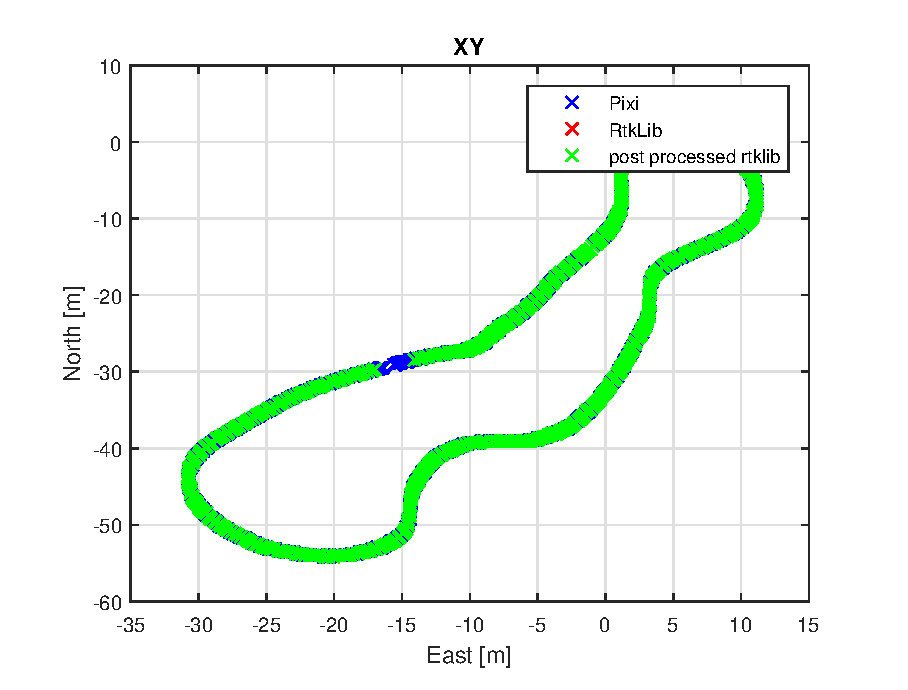
\includegraphics[width=0.7\textwidth]{figs/plots/xy.eps}
		\caption{A xy plot of the piksi,rtklib real time solution and the rtklib post processed solution}
		\label{figure:RTKLIB_STRUCTURE}
\end{figure}
\begin{figure}[H]
	\centering
		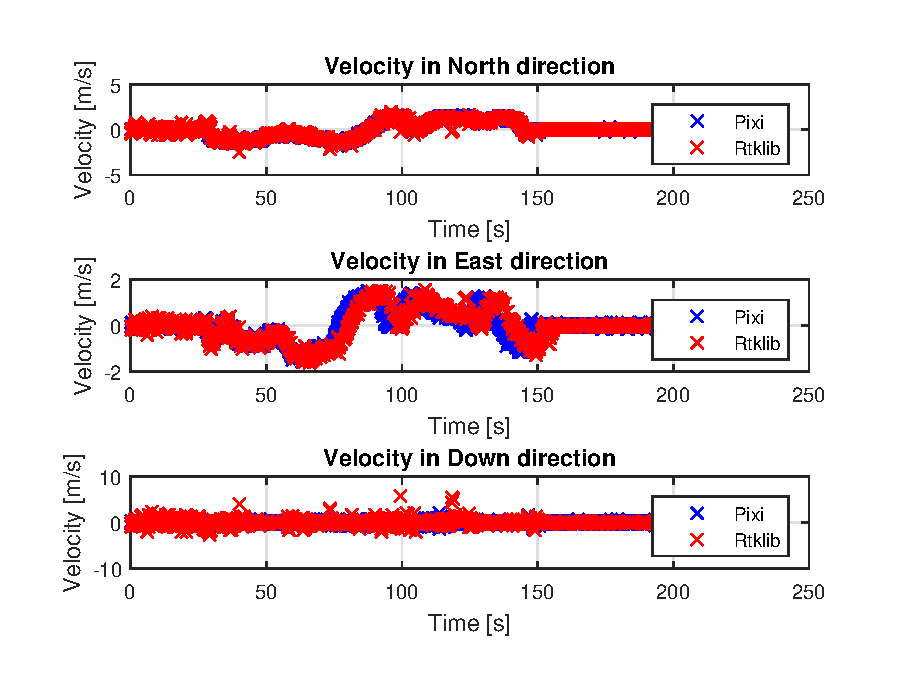
\includegraphics[width=0.7\textwidth]{figs/plots/velocity.eps}
		\caption{Velocity data from the piksi and rtklib real time solution}
		\label{figure:RTKLIB_STRUCTURE}
\end{figure}
\begin{figure}[H]
	\centering
		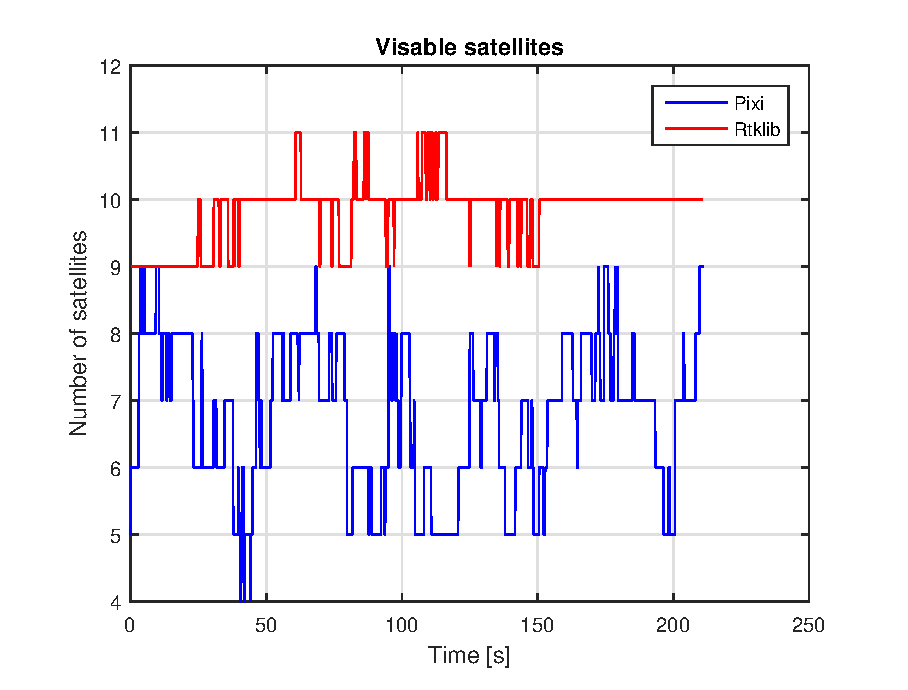
\includegraphics[width=0.7\textwidth]{figs/plots/sv.eps}
		\caption{Visable statellite for the piksi and rtklib}
		\label{figure:RTKLIB_STRUCTURE}
\end{figure}
\begin{figure}[H]
	\centering
		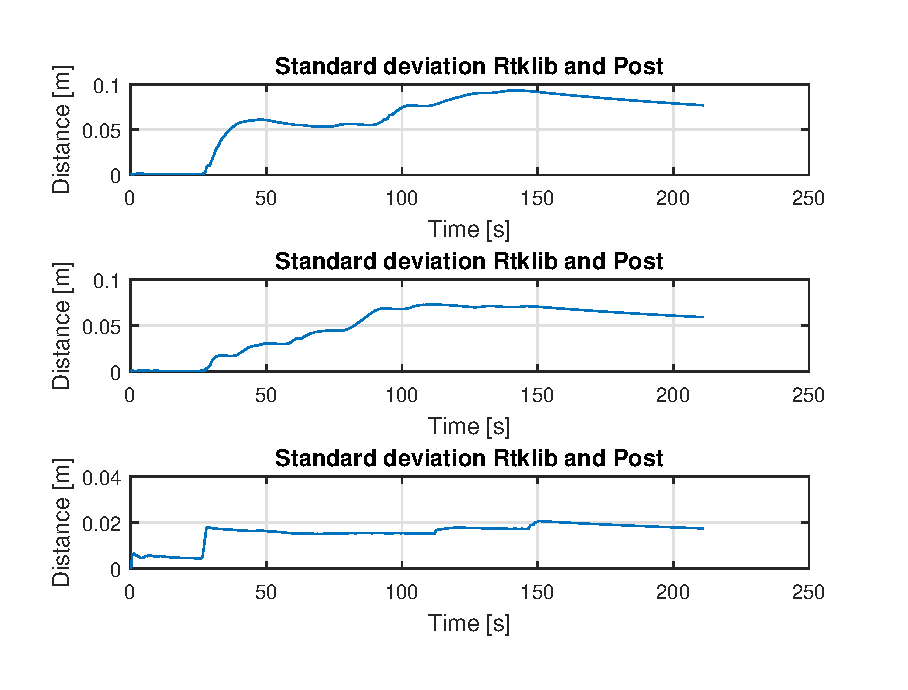
\includegraphics[width=0.7\textwidth]{figs/plots/stdrtkpost.eps}
		\caption{Standard deviation of the difference between rtklib real time and post processed solution}
		\label{figure:RTKLIB_STRUCTURE}
\end{figure}
\begin{figure}[H]
	\centering
		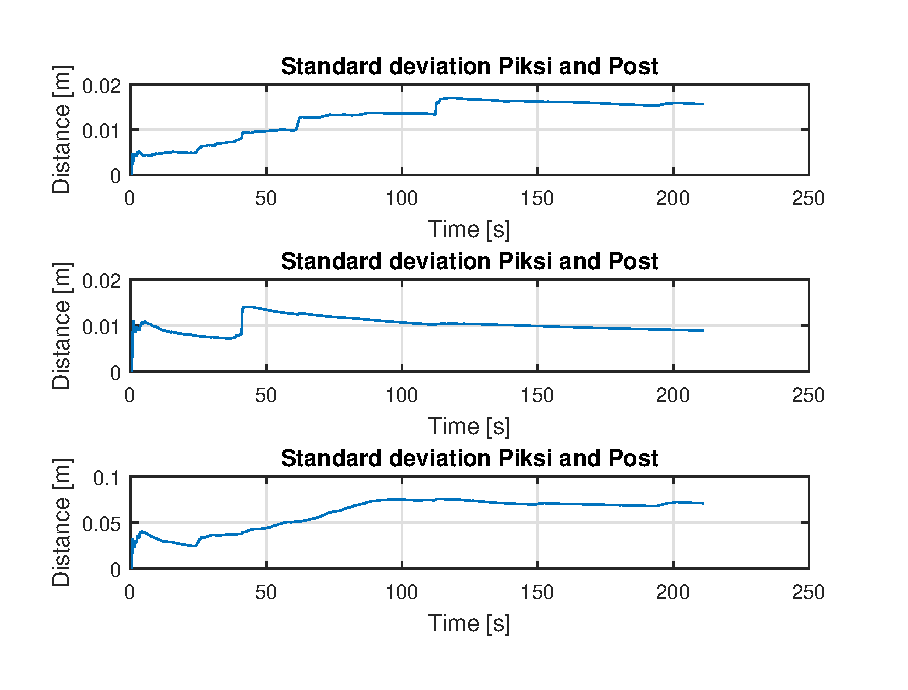
\includegraphics[width=0.7\textwidth]{figs/plots/stdpiksipost.eps}
		\caption{Standard deviation of the difference between piksi real time and rtklib post processed solution}
		\label{figure:RTKLIB_STRUCTURE}
\end{figure}
\begin{figure}[H]
	\centering
		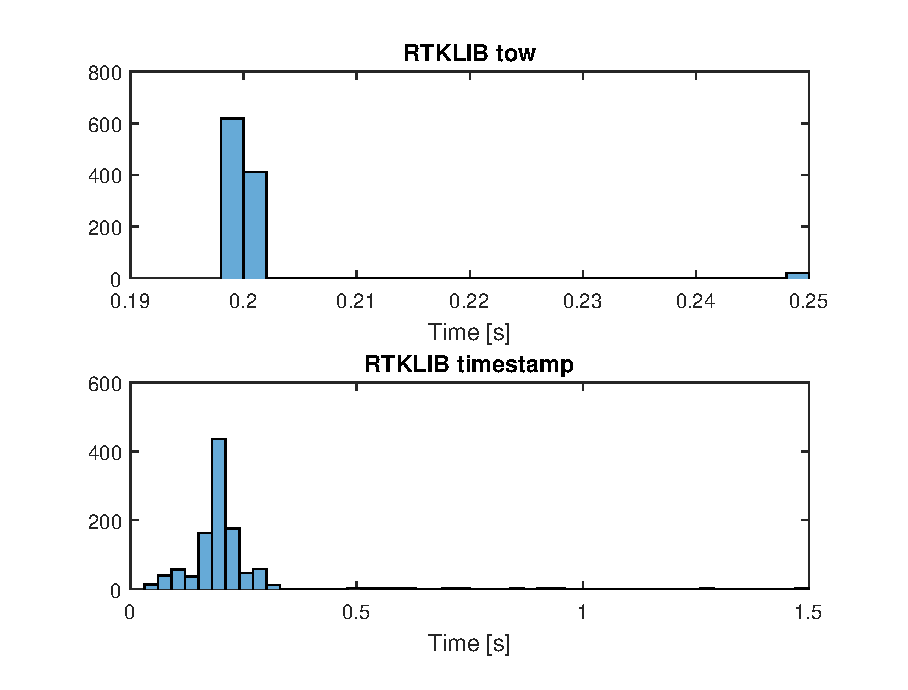
\includegraphics[width=0.7\textwidth]{figs/plots/rtktime.eps}
		\caption{The time between time samples from rtklib}
		\label{figure:RTKLIB_STRUCTURE}
\end{figure}
\begin{figure}[H]
	\centering
		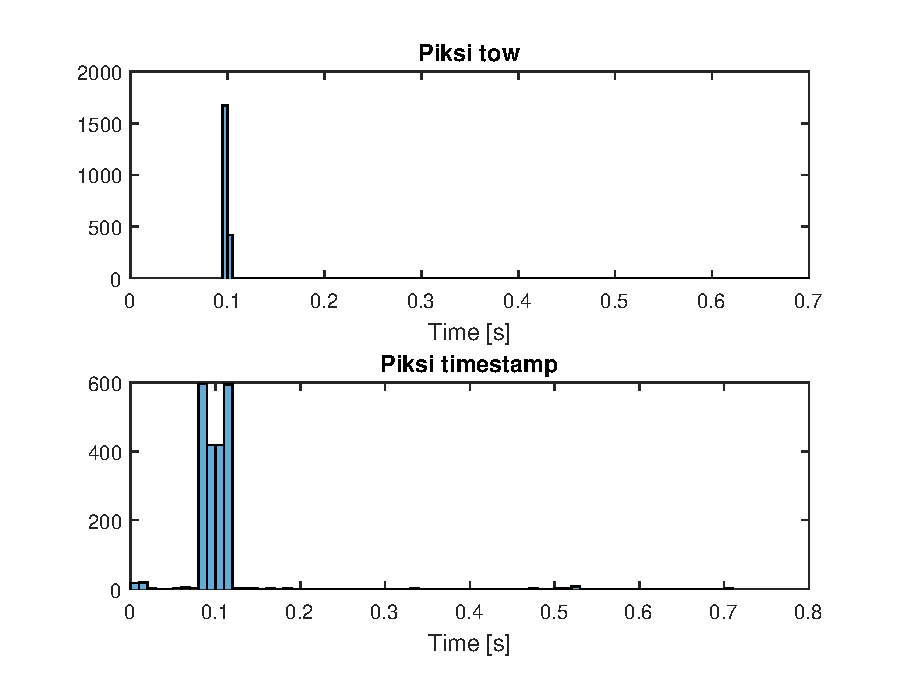
\includegraphics[width=0.7\textwidth]{figs/plots/piksitime.eps}
		\caption{The time between time samples from rtklib}
		\label{figure:RTKLIB_STRUCTURE}
\end{figure}
\begin{figure}[H]
	\centering
		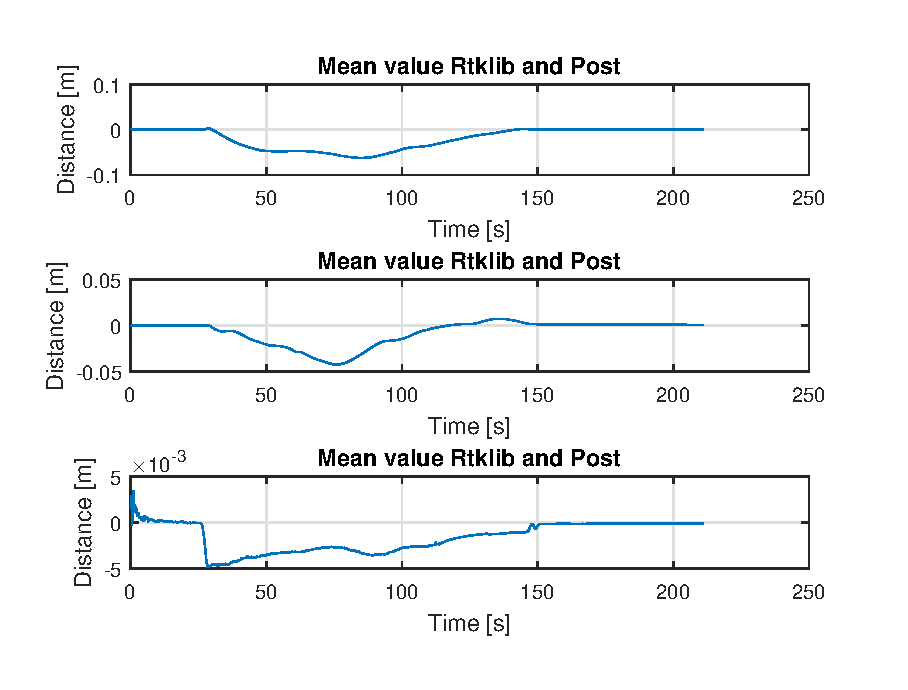
\includegraphics[width=0.7\textwidth]{figs/plots/meanrtkpost.eps}
		\caption{The mean difference between the rtklib real time and post processed solution}
		\label{figure:RTKLIB_STRUCTURE}
\end{figure}
\begin{figure}[H]
	\centering
		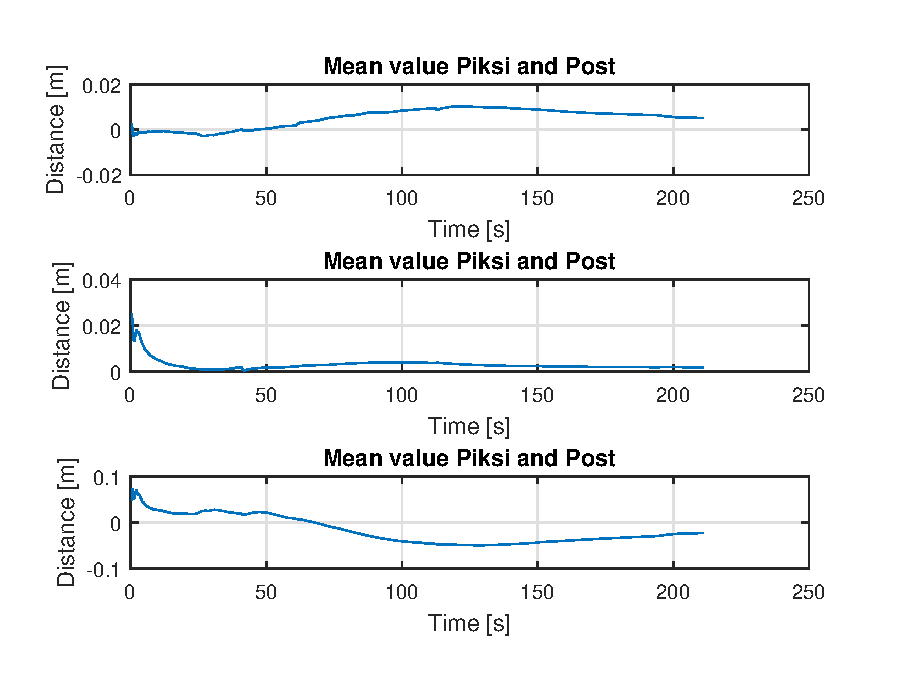
\includegraphics[width=0.7\textwidth]{figs/plots/meanpiksipost.eps}
		\caption{The mean difference between the piksi real time and the rtklib post processed solution}
		\label{figure:RTKLIB_STRUCTURE}
\end{figure}
\begin{figure}[H]
	\centering
		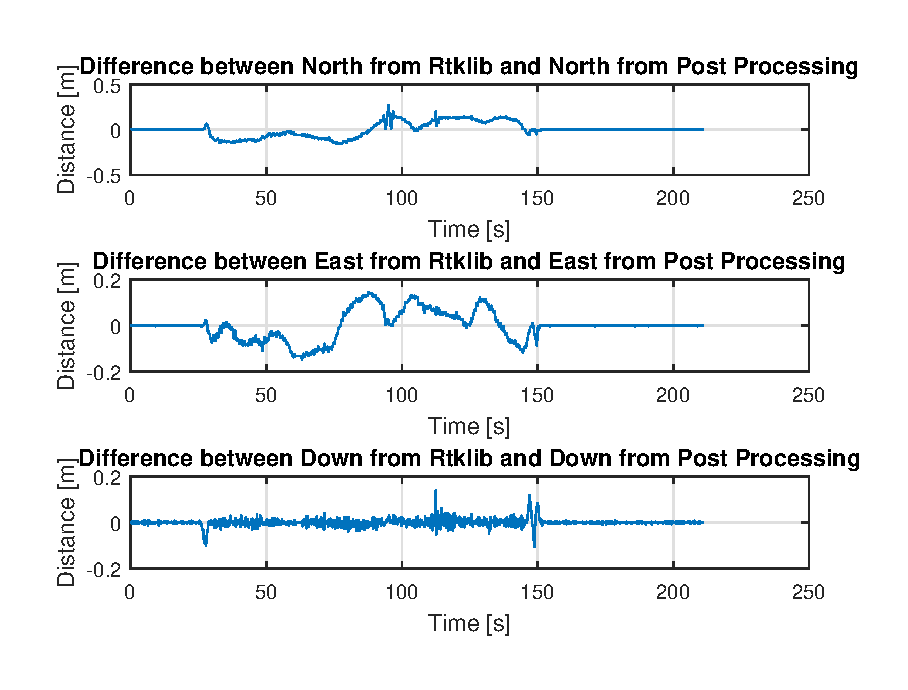
\includegraphics[width=0.7\textwidth]{figs/plots/ertkpost.eps}
		\caption{The difference between rtklib real time and post processed solution}
		\label{figure:RTKLIB_STRUCTURE}
\end{figure}
\begin{figure}[H]
	\centering
		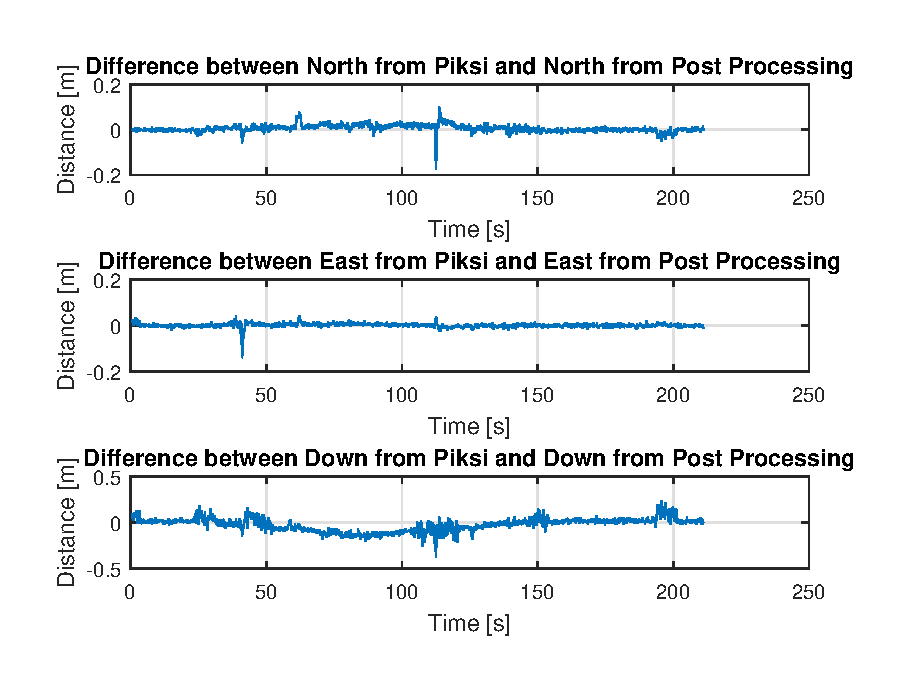
\includegraphics[width=0.7\textwidth]{figs/plots/epiksiport.eps}
		\caption{The communication structure of rtklib}
		\label{figure:RTKLIB_STRUCTURE}
\end{figure}
\begin{figure}[H]
	\centering
		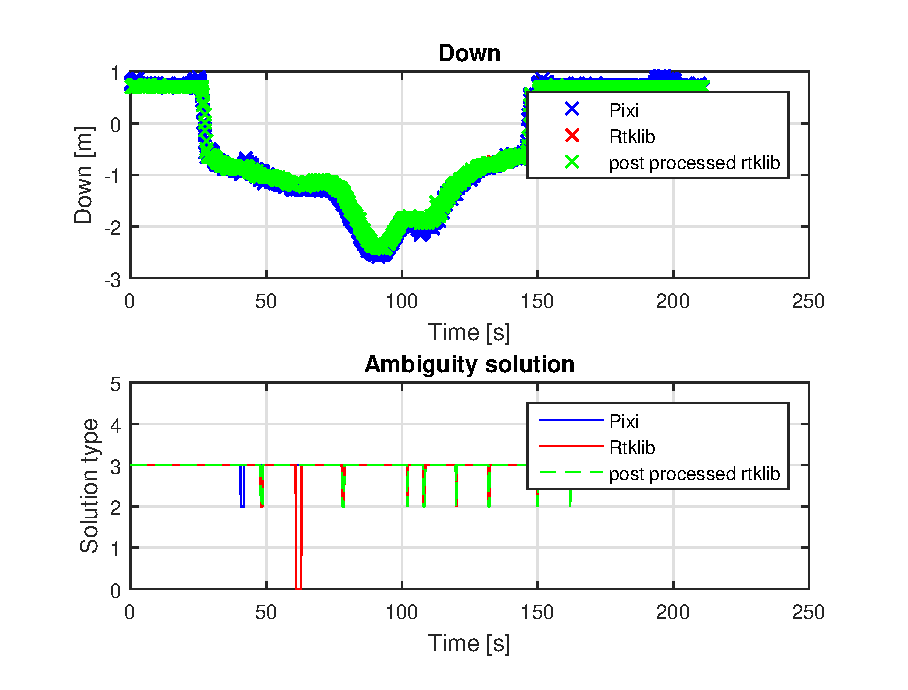
\includegraphics[width=0.7\textwidth]{figs/plots/down.eps}
		\caption{The communication structure of rtklib}
		\label{figure:RTKLIB_STRUCTURE}
\end{figure}
\cleardoublepage